% ----------------------------- CONCETTI AVANZATI ------------------------------------

\chapter{Concetti Avanzati}

% Argomenti di questo capitolo:

% unique pointers
% smart pointers
% shared pointer
% weak pointers
% friend functions
% e make unique

%TODO: Copy-and-Swap Idiom?
%TODO: Signal Handling? (magari in un capitolo sul multithreading)
%TODO: Prevent Object Copy?
%TODO: Command Line Arguments?

%TODO: tecniche per debuggare codice?
%TODO: Writing C++ code efficiently in Competitive Programming?

%TODO: 7 Advance C++ Concepts: RAII, Return Type Resolver, Type Erasure, CRTP, Virtual Constructor, SFINAE, Proxy.

%TODO: pointer to function?

% std uniform real distribution

% C++ 20: Concepts, ranges, coroutines, template parameter list, modules, ecc.. (non qui, ma in Le gemme della libreria degli Algoritmi)

%TODO: Dependency Injection
%TODO: std::static_pointer_cast
%TODO: std::enable_share_from_this
%TODO: allocate_shared
%TODO: Allocator
%TODO: std::bad_alloc

%TODO: std::clamp (non è chi sa che cosa di avanzato, comunque).
%TODO: normal_distribution

%TODO: magari aggiungere nel capitolo "basi del linguaggio": struct destructors che servono se allochi della memoria nelle struct, non se le usi, ma se allochi.

% -------------------------- SECTION: INTRODUZIONE -----------------------------------

\section{Introduzione}

\textsf{\small In questo capitolo "finale" tratterò argomenti un po' più complessi o che almeno non mi verrebbe da mettere negli altri due capitoli precedenti.} \\

\textsf{\small Verranno trattati argomenti come gli smart pointers e quindi unique pointers, share pointers, weak pointers, le friend function, uniform real distribution e altri importanti concetti avanzati.} \\

% -------------------------- SECTION: FRIEND KEYWORD ---------------------------------

\newpage

\section{Friend Keyword}

\subsection{Friend Class}

\textsf{\small \textbf{Definizione: } La keyword \textbf{friend} è usata per accedere ai membri privati e protetti di una classe nella quale è dichiarata \textbf{friend}.} \\

\begin{lstlisting}
	#include <iostream>
	
	class A {
		public:
			A() { a = 0 };
			friend class B; // Classe amica.
			
		private:
			int a;
	};

	class B {
		public:
			void showA(A& x)
			{
				// Visto che B è un'amica di A, può accedere ai membri privati di A.
				std::cout << "A::a : " << x.a; 
			}
	};

	int main()
	{
		A a;
		B b;
		b.showA(); //Output: A::a : 0
		return 0;
	}
\end{lstlisting}

\subsection{Friend Function}

\textsf{\small \textbf{Definizione: } Come per le \textbf{classi friend}, una \textbf{funzione friend} ha accesso speciale ai membri privati e protetti.} \\

\textsf{\small Una \textbf{friend function} può essere: } \\

\begin{itemize}
	\item \textsf{\small Un membro di un'altra classe.}
	\item \textsf{\small Una funzione globale.}
\end{itemize}

\textsf{\small Alcuni importanti punti riguardo alle \textbf{friend} functions e classes: } \\

\begin{itemize}
	\item \textsf{\small Dovrebbero essere usate solo in maniera limitata. Troppe funzioni o classi \textbf{friend} diminuiscono l'encapsulazione.}
	\item \textsf{\small L'amicizia non è reciproca. Se la classe A è amica della classe B, allora B non è automaticamente amica di A.}
	\item \textsf{\small L'amicizia non è ereditata.}
	%\item \textsf{\small }
\end{itemize}

\begin{lstlisting}
	#include <iostream>
	
	class A {
		public:
			friend void printWidth( A a);
			void setWidth(double w);
			
		private:
			double width;
	};

	// Definizione della funzione membro di A.
	void A::setWidth(double w)
	{
		width = w;
	}

	// printWidth non è una funzione membra di nessuna classe.
	void printWidth( A a )
	{
		// Visto che la funzione printWidth è amica di A, può accedere direttamente a qualsiasi membro di A.
		std::cout << "Width di A: " << a.width << std::endl;
	}

	int main()
	{
		A a;
		
		a.setWidth(11.1);
		
		// Uso la funzione amica per stampare la width di a.
		printWidth( a ) ; //Output: Width di A: 11.1
		return 0;
	}
\end{lstlisting}

% -------------------------- SECTION: SMART POINTERS ---------------------------------

\newpage

\section{Smart Pointers}

\textsf{\small \textbf{Definizione: } Gli \textbf{smart pointers} (puntatori intelligenti) sono dei puntatori che, in più rispetto ai normali puntatori, sono in grado deallocare la memoria automaticamente, senza che il programmatore debba occuparsene ed evitando \emph{memory leak}.} \\

\subsection{Differenze con i puntatori normali}

\textsf{\small I \textbf{puntatori} servono per poter accedere a delle risorse che sono esterne al programma (alla memoria heap). Grazie ai puntatori saremo in grado di modificare direttamente la risorsa esterna, al posto di doverne fare una copia.} \\

\textsf{\small Il problema di questi puntatori è che se non deallocati correttamente potrebbero portare ad uno spreco della memoria heap, il che è un \emph{memory leak}.} \\

\begin{lstlisting}
	#include <iostream>
	
	class Rectangle {
		private:
			int width;
			int height;
	};

	void fun()
	{
		Rectangle* p = new Rectangle();
	}

	int main()
	{
		while(1)
		{
			fun();
		}
		//Output: Il problema è che quando la funzione fun termina, il puntatore p verrà distrutto come fosse una variabile locale, ma la memoria allocata non verrà deallocata, perché ci siamo scordati di usare \emph{delete p}; alla fine della funzione.
		
		// Ciò è un problema perché verrà sempre allocata altra memoria e mai deallocata, occupando spazio, sprecando memoria, il che è un \emph{memory leak}.
		
		// L'intera memoria heap potrebbe diventare inutile per questo motivo. 
		return 0;
	}
\end{lstlisting}

\textsf{\small Il problema è che quando la funzione fun termina, il puntatore p verrà distrutto come fosse una variabile locale, ma la memoria allocata non verrà deallocata, perché ci siamo scordati di usare \emph{delete p}; alla fine della funzione.} \\

\textsf{\small Ciò è un problema perché verrà sempre allocata altra memoria e mai deallocata, occupando spazio, sprecando memoria, il che è un \emph{memory leak}.} \\

\textsf{\small L'intera memoria heap potrebbe diventare inutile per questo motivo. } \break

\textsf{\small Uno \textbf{smart pointer} è un \emph{wrapper} (un wrapper è un'entità che ne encapsula un'altra; è del codice che letteralmente avvolge, incarta, impacchetta, confeziona dell'altro codice) su un puntatore con un'operatore \textbf{*} e \textbf{->} overloaded.} \\

\textsf{\small La memoria allocata dinamicamente verrebbe così automaticamente liberata.} \\

\begin{lstlisting}
	// Una generica classe Smart Pointer
	#include <iostream>
	
	template <class T>
	class SmartPointer {
		T *ptr;
		public:
			SmartPointer(T *ptr = NULL)
			{
				p = ptr;
			}
		
			~SmartPointer()
			{
				delete ptr;
			}
		
			T & operator * ()
			{
				return *ptr;
			}
		
			T * operator ->()
			{
				return ptr;
			}
	};

	int main()
	{
		SmartPointer<int> p(new int());
		*p = 22;
		std::cout << "Valore di *p: " << *p << std::endl; //Output: Valore di *p: 22
		return 0;
	}
\end{lstlisting}

%TODO: unique, share, weak, 
%TODO: std::make_unique vs std::unique_ptr
%TODO: std::make_shared

%TODO: problemi dei vecchi puntatori.

%TODO: std::static_pointer_cast
%TODO: std::enable_share_from_this
%TODO: allocate_shared
%TODO: Allocator
%TODO: std::bad_alloc
%TODO: auto_ptr (C++98)

\subsection{unique pointers}

\textsf{\small \textbf{Definizione: } Gli \textbf{unique pointers} sono un tipo di \textbf{smart pointers} che memorizzano un solo puntatore alla volta.} \\

\textsf{\small Sarà necessario includere \textbf{<memory>} per poter usufruire degli \textbf{unique pointers}.} \\

\begin{lstlisting}
	#include <iostream>
	#include <memory> // Per gli unique pointers, ecc..
	
	// Per dichiarare un unique pointer
	std::unique_ptr<int> p(new int(3));
\end{lstlisting}

\begin{figure}[H]
	\centering
	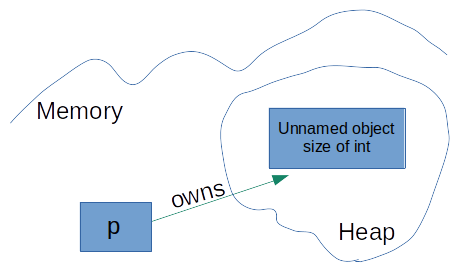
\includegraphics[width=1\textwidth, height=1\textheight, keepaspectratio]{./imgs/unique_ptr_definition.png}
	\caption{Unique ptr}
	\label{fig:unique_ptr_definition}
\end{figure}

\textsf{\small Se lo \textbf{unique\_ptr} viene distrutto, anche la memoria allocata nell'heap viene distrutta di conseguenza.} \\

\begin{figure}[H]
	\centering
	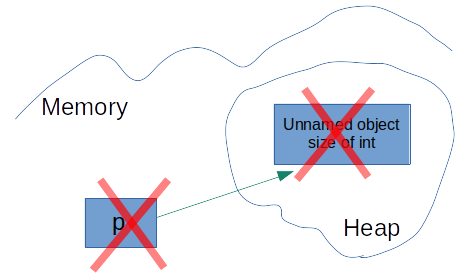
\includegraphics[width=1\textwidth, height=1\textheight, keepaspectratio]{./imgs/unique_ptr_delete.png}
	\caption{Unique ptr delete}
	\label{fig:unique_ptr_delete}
\end{figure}

\textsf{\small Per creare uno \textbf{unique\_ptr} si può anche utilizzare \textbf{std::make\_unique}.} \\

\begin{lstlisting}
	#include <iostream>
	
	class Rectangle {
		public:
			Rectangle(int w, int h)
			{
				this->width = w;
				this->height = h;
			}
		
			int area()
			{
				return width * height;
			}
		
		private:
			int width;
			int height;
	};

	int main()
	{
		auto pRect = std::make_unique<Rectangle>(3, 4);
		std::cout << "Area del rettangolo: " << pRect->area() << std::endl; //Output: Area del rettangolo: 12
		return 0;
	}
\end{lstlisting}

\subsubsection{Differenza tra std::make\_unique vs std::unique\_ptr}

\textsf{\small Ci sono varie ragioni per cui utilizzare \textbf{std::make\_unique} al posto di \textbf{std::unique\_ptr} con la new: } \\

\begin{itemize}
	\item \textsf{\small È sicuro nel caso si vogliano creare dei temporanei, mentre con la new ti devi ricordare la reogla: del non usare temporanei senza nome. } 
	\item \textsf{\small Con l'utilizzo di \textbf{make\_unique} si può finalmente evitare di usare la \textbf{new}, a differenza della vecchia regola: mai usare la \textbf{new} tranne per gli \textbf{unique\_ptr}.} 
	\item \textsf{\small Non richiede \emph{type usage} ridondante: \emph{unique\_ptr<T>(new T())} -> make\_unique<T>().} \\
	\item \textsf{\small Così da non dover esplicitare gli argomenti dei \emph{template types}.}
	\item \textsf{\small Aggiunge sicurezza riguardo le eccezioni.}
	\item \textsf{\small Altrimenti non potresti accedere al costruttore della classe fuori dallo \emph{scope} corrente.}
	%\item \textsf{\small }
\end{itemize}

\subsubsection{Ownership | move}

\textsf{\small Un \textbf{unique pointer} è una relazione 1 a 1 con l'oggetto allocato.} \\

\textsf{\small Non può essere copiato o passato per valore, però la \textbf{ownership} (proprietà) dell'oggetto può essere trasferita.} \\

\begin{lstlisting}
	#include <iostream>
	
	class Person {
		public:
			Person(std::string s) : name(s) {};
			~Person() { std::cout << "Libero spazio" << std::endl };
			
			std::string getName() { return this->name };
			
		private:
			std::string name;
	};

	int main()
	{
		auto ptrPerson = std::make_unique<Person>("Luigi");
		
		std::cout << "Nome: " << ptrPerson->getName() << std::endl; //Output: Nome: Luigi
		
		std::unique_ptr<Person> ptrPerson2;
		
		ptrPerson2 = std::move(ptrPerson);
		
		std::cout << "Nome: " << ptrPerson2->getName() << std::endl; //Output: Nome: Luigi
		
		std::cout << "Nome dopo il trasferimento dell'ownership: " << ptrPerson->getName() << std::endl; //Output: [non stampa niente]
		
		return 0;
	}
\end{lstlisting}

\begin{figure}[H]
	\centering
	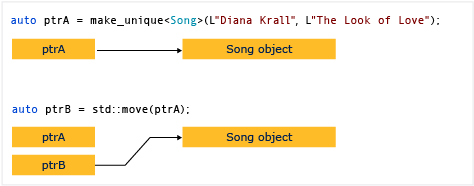
\includegraphics[width=1\textwidth, height=1\textheight, keepaspectratio]{./imgs/unique_ptr_move2.png}
	\caption{Unique ptr move}
	\label{fig:unique_ptr_move2}
\end{figure}

\subsubsection{Operazioni sugli unique\_ptr}

\textsf{\small Varie operazioni sono supportate sugli \textbf{unique\_ptr}: } \\

\begin{itemize}
	\item \textsf{\small \textbf{*} : Dereferenza del puntatore.}
	\item \textsf{\small \textbf{->} : Accedere ai membri della classe.}
	\item \textsf{\small \textbf{.get()} : per ottenere il \emph{raw pointer} del \textbf{unique\_ptr} (non cancellarlo, perché è gestito dal unique pointer; è da usare solo per calcoli).}
	\item \textsf{\small \textbf{.reset(new int())} : cancella il vecchio oggetto e ne crea uno nuovo (al posto di new int() avremmo potuto passare qualsiasi altro oggetto, era per fare un esempio).}
	\item \textsf{\small \textbf{move} : trasferisce la proprietà del \textbf{unique\_ptr}.}
	\item \textsf{\small \textbf{swap} : per scambiare due \textbf{unique pointers}.}
	\item \textsf{\small \textbf{if(unique\_ptr)} : se passiamo uno \textbf{unique\_ptr} all'if restituisce falso se non è associato a nessun oggetto.}
	%\item \textsf{\small \textbf{} : }
\end{itemize}

\subsubsection{Passare uno unique\_ptr ad una funzione}

\textsf{\small Utilizziamo \textbf{std::move} per trasferire la proprietà del \textbf{unique\_ptr}.} \\

\begin{lstlisting}
	#include <iostream>
	#include<memory>
	
	struct A {
		int x;
		~A() { std::cout << "Libero spazio" << std::endl };
	};

	void passUniquePtr(std::unique_ptr<A> a)
	{
		// Usciti dalla funzione lo unique\_ptr e il suo oggetto vengono cancellati, perché locali alla funzione.
		std::cout << "Puntatore ricevuto" << '\n';
		a->x = 5;
		std::cout << "a.x: " << a->x << std::endl;
	}

	int main()
	{
		auto ptrA = std::make_unique<A>();
		passUniquePtr(std::move(ptrA));
		
		// true = ptrA è vuoto.
		if(!ptrA)
		{
			std::cout << "ptrA è vuoto" << std::endl;
		}
	
		//Output: Puntatore ricevuto
		//Output: a.x: 5
		//Output: Libero spazio
		//Output: ptrA è vuoto
		return 0;
	}
\end{lstlisting} 

\subsubsection{Restituire un unique\_ptr}

\textsf{\small Si può restituire uno \textbf{unique\_ptr} da una funzione. } \\

\begin{lstlisting}
	#include <iostream>
	#include <memory>
	
	class A {};
	
	std::unique_ptr<A> returnUniquePtr()
	{
		auto a = std::make_unique<A>();
		return a;
	}

	int main()
	{
		auto ptrA = returnUniquePtr();
		
		if(ptrA)
		{
			std::cout << "ptrA ha un oggetto. " << std::endl;	
		}
	
		//Output: ptrA ha un oggetto.
		return 0;
	}
\end{lstlisting}

\subsubsection{Membri delle classi: unique pointer vs raw pointer vs reference}

\textsf{\small } \\

\begin{itemize}
	\item \textsf{\small \textbf{Unique pointer membro della classe} : la classe è la proprietaria dell'oggetto del puntatore.}
	\item \textsf{\small \textbf{Raw pointer membro della classe} : La classe è un osservatore e non è responsabile di rimuovere l'oggetto puntato dal puntatore. Viene rimosso da uno smart pointer fuori dalla classe.}
	\item \textsf{\small \textbf{Referenza membro della classe} : è garantito che la referenza contiene dati validi mentre la classe è "viva".}
	%\item \textsf{\small }
\end{itemize}

%TODO: std::make_unique
%TODO: operazioni possibili sugli unique pointers
%TODO: std::move, move ownership
%TODO: std::swap
%TODO: pass as an argument
%TODO: return it from a function


\subsection{share pointers}

\textsf{\small \textbf{Definizione: } } \\

\subsection{weak pointers}

\textsf{\small \textbf{Definizione: } } \\

% -------------------------- SECTION: UNIFORM REAL DISTRIBUTION ----------------------

\newpage

\section{Uniform Real Distribution}

\textsf{\small \textbf{Definizione: } } \\

%TODO: Dependency Injection

% -------------------------- SECTION: 7 CONCETTI AVANZATI ----------------------------

\newpage

%TODO: Questo come ultimo argomento del capitolo!

%TODO: Come prima cosa qui aggiungere quell'immagine sui 7 concetti avanzati.

%TODO: RAII, Return Type Resolver, Type Erasure, CRTP, Virtual Constructor, SFINAE, Proxy.

\section{7 Concetti Avanzati}

\subsection{RAII}

\textsf{\small \textbf{Definizione: } } \\ %TODO: scrivere che abbiamo già trattato questo argomento nel precedente capitolo oppure nel capitolo Concetti Intermedi, ma voglio comunque ripassarlo qui.

\subsection{Return Type Resolver}

\subsection{Type Erasure}

\subsection{CRTP}

\subsection{Virtual Constructor}

\subsection{SFINAE}

%TODO: tratterò questo argomento anche nel capitolo Le gemme della libreria degli Algoritmi.

\subsection{Proxy}

% ------------------------------------------------------------------------------------